\documentclass[aspectratio=169]{beamer}
\usepackage[utf8]{inputenc}
\usepackage{lmodern}
\usepackage{tikz}
\usepackage{hyperref}
\usetikzlibrary{positioning,arrows.meta}
\definecolor{neonblue}{HTML}{2F80ED}
\definecolor{mango}{HTML}{F2994A}
\definecolor{violet}{HTML}{7B61FF}
\definecolor{mint}{HTML}{27AE60}
\definecolor{ink}{HTML}{17212F}
\definecolor{panel}{HTML}{F6F9FF}
\setbeamertemplate{navigation symbols}{}
\setbeamercolor{normal text}{fg=ink,bg=white}
\setbeamercolor{frametitle}{fg=ink,bg=white}
\setbeamercolor{block title}{fg=white,bg=violet}
\setbeamercolor{block body}{fg=ink,bg=panel}
\setbeamertemplate{itemize item}{\color{neonblue}$\blacktriangleright$}
\setbeameroption{hide notes}
\title{Design Operating Systems | Day 2: Troubleshooting}
\subtitle{Student Mission Deck}
\author{Pine Brook IGNITE}
\date{Spring 2026}
\begin{document}

\begin{frame}[plain]
\begin{tikzpicture}[remember picture,overlay]
\fill[panel] (current page.south west) rectangle (current page.north east);
\fill[violet!16] (0.3,0.6) rectangle (13.0,6.9);
\draw[line width=7pt, color=neonblue] (0.55,6.65) -- (12.75,6.65);
\draw[line width=7pt, color=mango] (0.55,0.85) -- (12.75,0.85);
\end{tikzpicture}
\vspace{0.5cm}
\begin{center}
{\Huge\bfseries\color{ink} Design Operating Systems | Day 2: Troubleshooting\par}
\vspace{0.18cm}
{\Large\color{violet} Mission Board: Learn, Test, Improve.\par}
\vspace{0.28cm}

\begin{tikzpicture}
\node[rounded corners=18pt, fill=white, draw=neonblue, line width=1.4pt, minimum width=10.8cm, minimum height=1.5cm, text width=9.9cm, align=center]
{\Large\bfseries Intermediate learners benefit from a clear mission board, visible debugging routine, and fewer hidden setup steps.};
\end{tikzpicture}
\vspace{0.32cm}
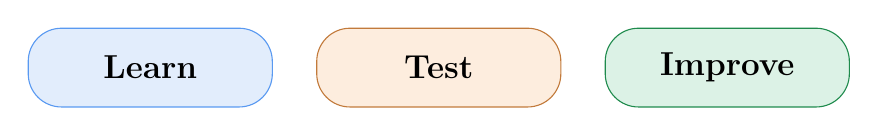
\begin{tikzpicture}[node distance=0.55cm]
\node[rounded corners=12pt, fill=neonblue!14, draw=neonblue!80, minimum width=3.1cm, minimum height=1.0cm, align=center] (a) {\large\bfseries Learn};
\node[rounded corners=12pt, fill=mango!18, draw=mango!80!black, minimum width=3.1cm, minimum height=1.0cm, align=center, right=of a] (b) {\large\bfseries Test};
\node[rounded corners=12pt, fill=mint!16, draw=mint!80!black, minimum width=3.1cm, minimum height=1.0cm, align=center, right=of b] (c) {\large\bfseries Improve};
\end{tikzpicture}
\end{center}
\note{Today we are working on design operating systems |}
\end{frame}

\begin{frame}[plain]
\frametitle{Mission Brief}
\begin{columns}[T,totalwidth=\textwidth]
\column{0.55\textwidth}
\begin{block}{Your mission today}
\Large - I can determine possible solutions to solve common chromebook problems (troubleshooting).
\end{block}
\begin{itemize}\large
\item - I can determine possible solutions to solve common chromebook problems (troubleshooting).
\item I can make or improve something.
\item I can show my learning.
\end{itemize}
\column{0.4\textwidth}
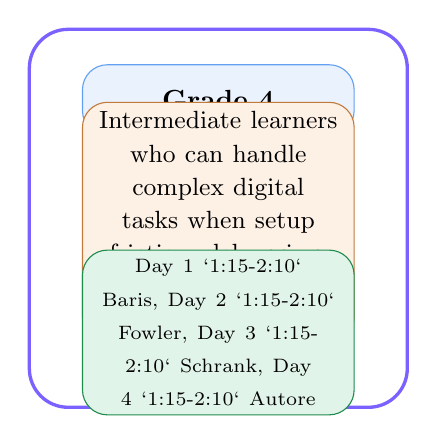
\begin{tikzpicture}[x=1cm,y=1cm]
\draw[rounded corners=14pt, fill=white, draw=violet, line width=1.2pt] (0,0) rectangle (4.8,4.8);
\node[draw=neonblue!75, fill=neonblue!10, rounded corners=9pt, minimum width=3.45cm, minimum height=0.9cm] at (2.4,3.9) {\bfseries Grade 4};
\node[draw=mango!80!black, fill=mango!14, rounded corners=9pt, minimum width=3.45cm, minimum height=1.05cm, text width=3.1cm, align=center] at (2.4,2.35) {\small Intermediate learners who can handle complex digital tasks when setup friction, debugging, and persistence are explicitly coached.};
\node[draw=mint!80!black, fill=mint!14, rounded corners=9pt, minimum width=3.45cm, minimum height=0.95cm, text width=3.1cm, align=center] at (2.4,0.95) {\scriptsize Day 1 `1:15-2:10` Baris, Day 2 `1:15-2:10` Fowler, Day 3 `1:15-2:10` Schrank, Day 4 `1:15-2:10` Autore};
\end{tikzpicture}
\end{columns}
\note{Today we are working on design operating systems |}
\end{frame}

\begin{frame}[plain]
\frametitle{Mission Flow}
\begin{center}
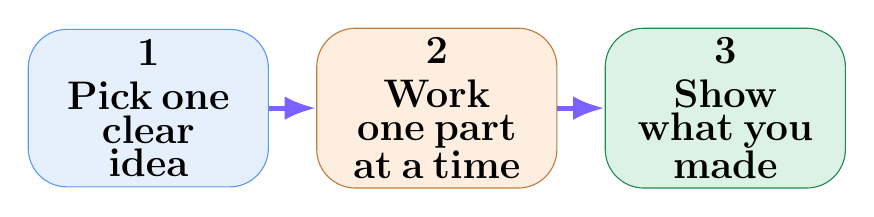
\begin{tikzpicture}[node distance=0.6cm]
\node[rounded corners=14pt, fill=neonblue!12, draw=neonblue!80, minimum width=3.05cm, minimum height=2.0cm, text width=2.3cm, align=center] (s1) {\Large\bfseries 1\\[4pt]Pick one clear idea};
\node[rounded corners=14pt, fill=mango!17, draw=mango!80!black, minimum width=3.05cm, minimum height=2.0cm, text width=2.3cm, align=center, right=of s1] (s2) {\Large\bfseries 2\\[4pt]Work one part at a time};
\node[rounded corners=14pt, fill=mint!16, draw=mint!80!black, minimum width=3.05cm, minimum height=2.0cm, text width=2.3cm, align=center, right=of s2] (s3) {\Large\bfseries 3\\[4pt]Show what you made};
\draw[-{Latex[length=4mm,width=3mm]}, line width=1.8pt, color=violet] (s1) -- (s2);
\draw[-{Latex[length=4mm,width=3mm]}, line width=1.8pt, color=violet] (s2) -- (s3);
\end{tikzpicture}
\end{center}
\vspace{0.3cm}
\begin{block}{Tools and setup}
\begin{itemize}\large
\item Begin by naming the lesson purpose and the success condition
\item Model the first step before independent or partner work starts
\item Pause once mid-lesson for a quick debug, reflection, or reset
\end{itemize}
\end{block}
\note{Use the help routine before you panic}
\end{frame}

\begin{frame}[plain]
\frametitle{Debug and Get Unstuck}
\begin{columns}[T,totalwidth=\textwidth]
\column{0.53\textwidth}
\begin{block}{Use this order}
\begin{enumerate}\large
\item Re-check the goal.
\item Re-check the current step.
\item Test one small change.
\item Ask one specific question.
\end{enumerate}
\end{block}
\column{0.42\textwidth}
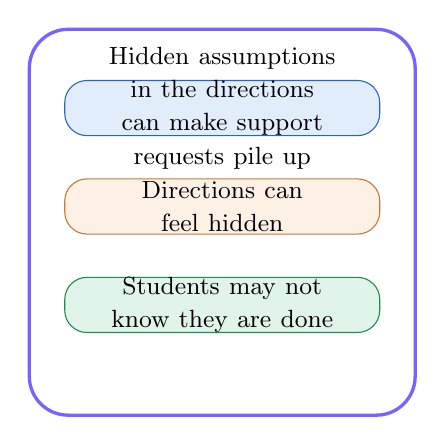
\begin{tikzpicture}[x=1cm,y=1cm]
\draw[rounded corners=14pt, fill=white, draw=violet, line width=1.2pt] (0,0) rectangle (4.9,4.9);
\foreach \y/\txt/\col in {3.9/Hidden assumptions in the directions can make support requests pile up/neonblue,2.65/Directions can feel hidden/mango,1.4/Students may not know they are done/mint} {
  \draw[rounded corners=8pt, fill=\col!14, draw=\col!80!black] (0.45,\y-0.35) rectangle (4.45,\y+0.35);
  \node[text width=3.4cm, align=center] at (2.45,\y) {\small \txt};
}
\end{tikzpicture}
\end{columns}
\note{Use the help routine before you panic}
\end{frame}

\begin{frame}[plain]
\frametitle{Proof of Learning}
\begin{center}
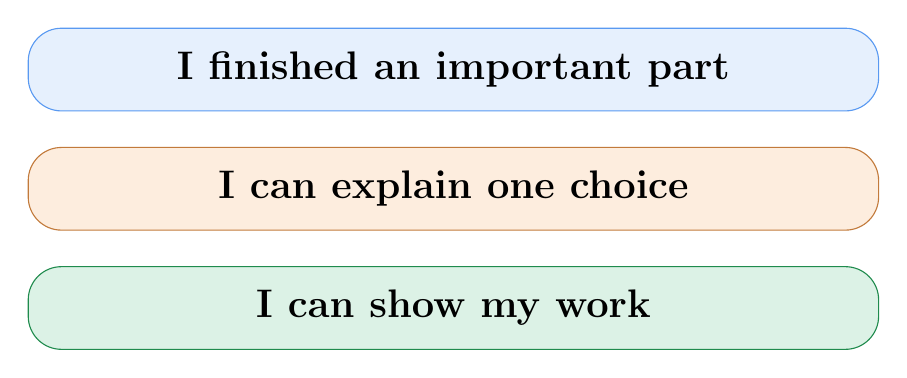
\begin{tikzpicture}[node distance=0.45cm]
\node[rounded corners=12pt, fill=neonblue!12, draw=neonblue!80, minimum width=10.8cm, minimum height=1.05cm, align=center] (a) {\Large\bfseries I finished an important part};
\node[rounded corners=12pt, fill=mango!18, draw=mango!80!black, minimum width=10.8cm, minimum height=1.05cm, align=center, below=of a] (b) {\Large\bfseries I can explain one choice};
\node[rounded corners=12pt, fill=mint!16, draw=mint!80!black, minimum width=10.8cm, minimum height=1.05cm, align=center, below=of b] (c) {\Large\bfseries I can show my work};
\end{tikzpicture}
\end{center}
\vspace{0.3cm}
\begin{block}{Before you leave}
\Large Save it, share it, explain it, or demonstrate it.
\end{block}
\note{Show what you learned at the end}
\end{frame}

\end{document}
